\chapter{Sequential kinematic simulation of multi-DOF reconfigurable trusses}\label{apdx-sequential-kinematics}
This section outlines the method for developing a sequential kinematic simulation program (attached as Supplementary Material), which enables the movement of one degree of freedom at a time in any reconfigurable truss generated by the workflow in Section~\ref{subsec-algo}. The reconfigurable trusses in this study consist of two types of units, each with a single degree of freedom (DOF): \mbox{(\textit{i}\hspace{.5pt})} a Grashof quadrilateral linkage; and \mbox{(\textit{ii}\hspace{.5pt})} a unique configuration of a six-bar linkage. The kinematic simulator performs the position analysis of one DOF at a time, while  applying rigid rotation and translation to the structure excluding DOFs that were actuated in previous steps. The position analysis for the two types of units is performed as follows.

\begin{figure}[!htbt]
  \centering
  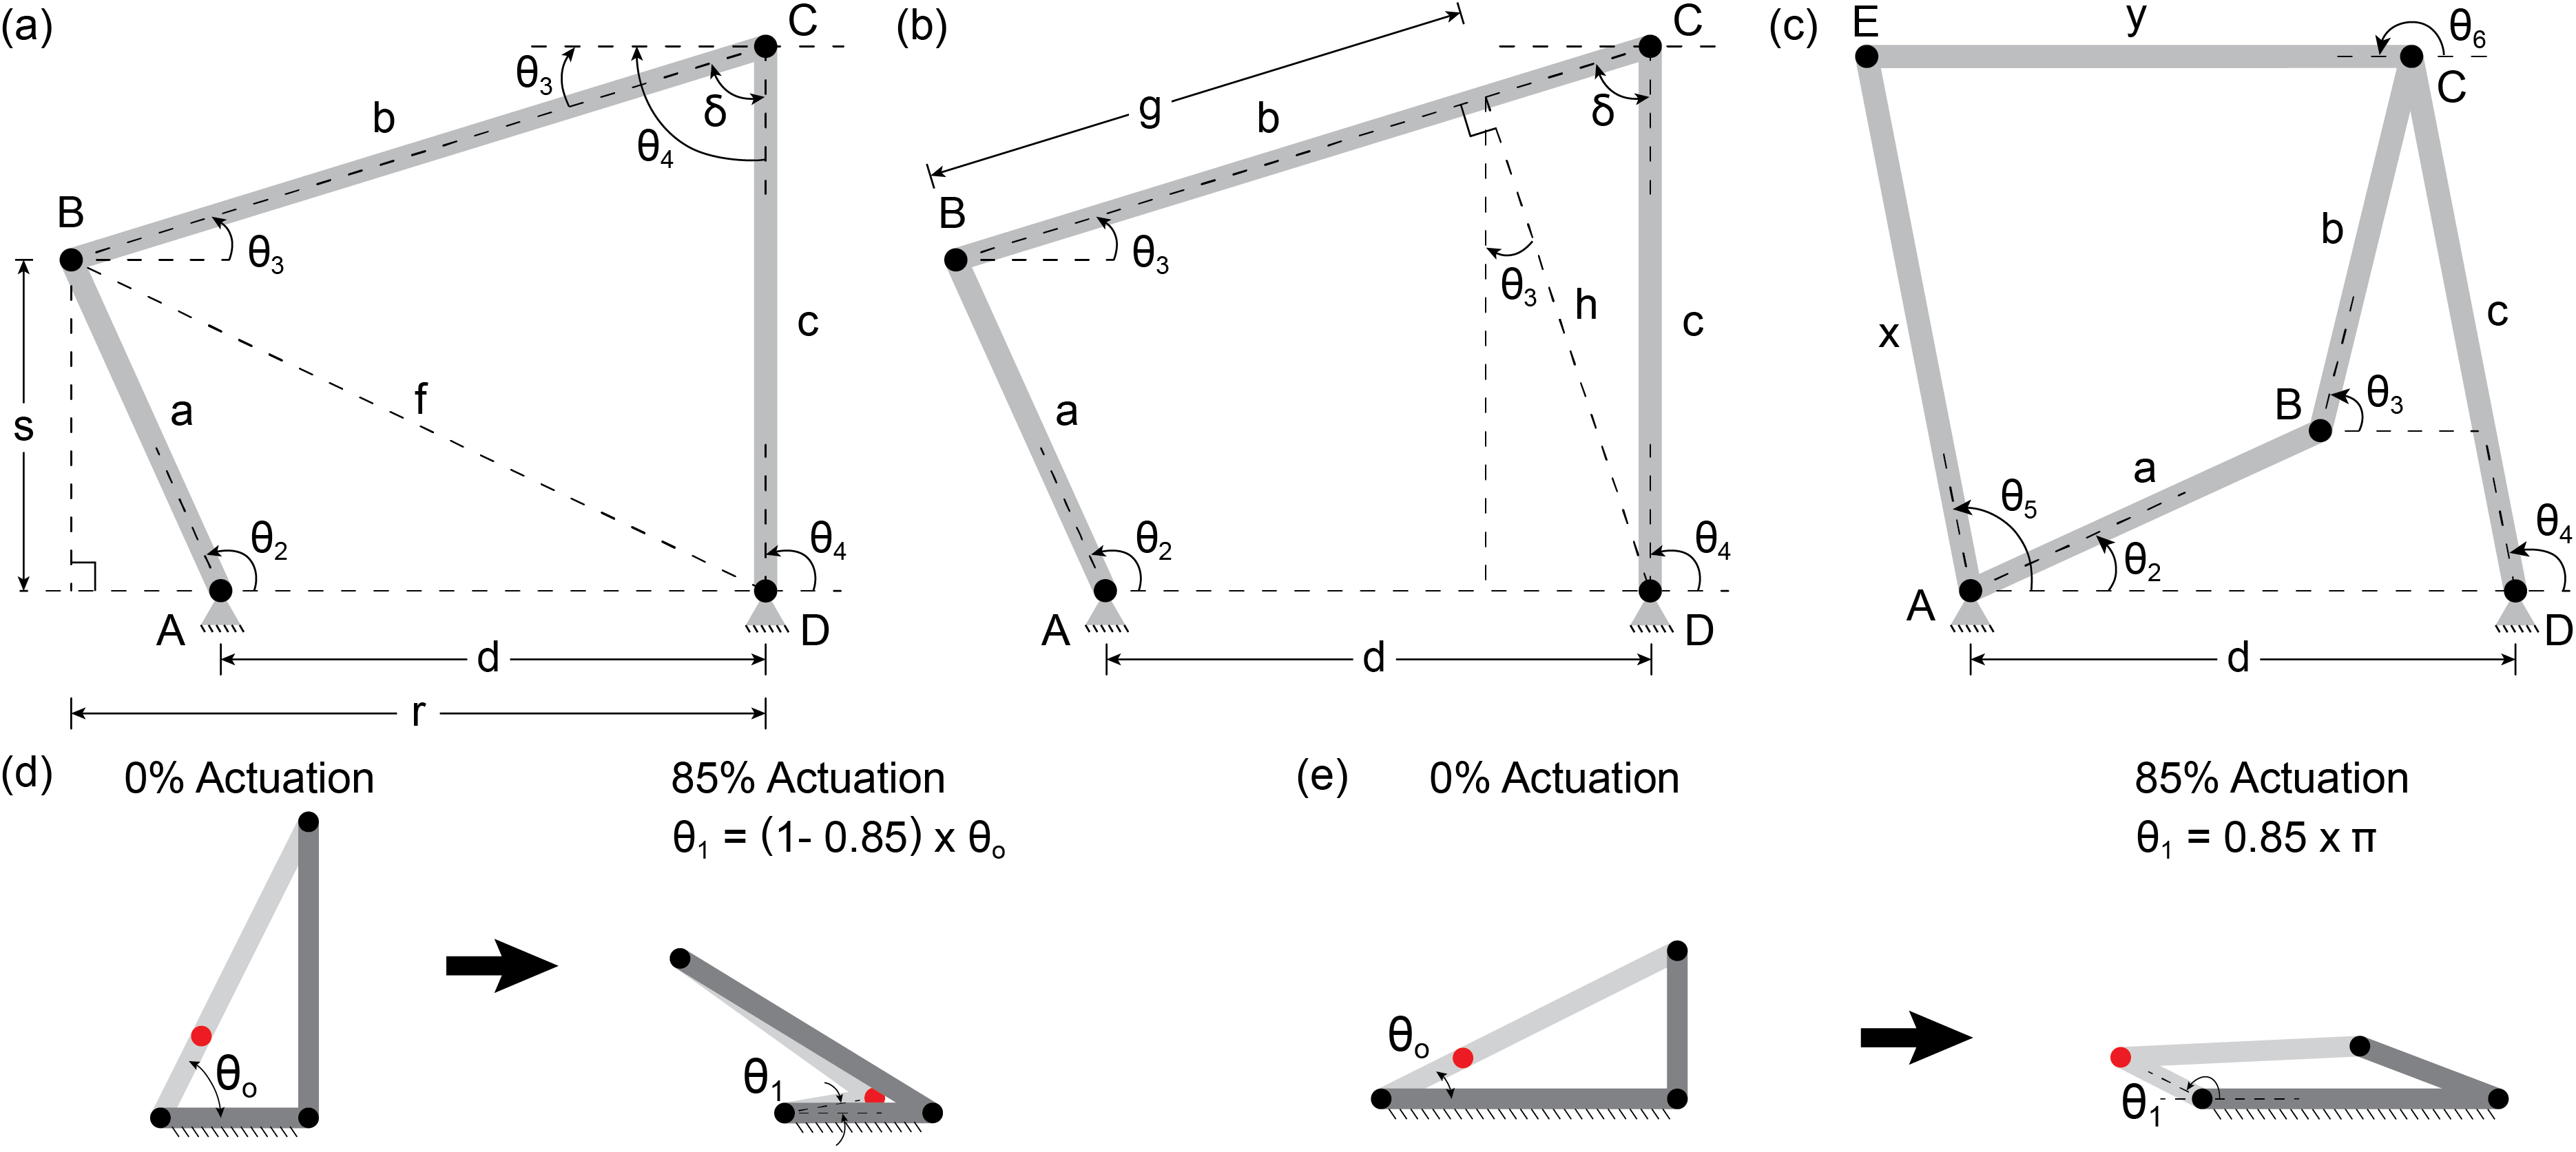
\includegraphics[width=\textwidth]{01-figures/a1-linkage-kinematics-190mm.jpg}
  \caption{Position analysis using the Method of Projections for: (a-b) a general quadrilateral linkage; (c) a unique configuration of a six-bar linkage; (d-e) Extent of actuation in terms of \% actuation of the DOF explained for two different geometries of quadrilateral linkage. \textbf{Note:} A Ground link is not explicitly shown in (a)-(c) but is assumed to be present between nodes A and D.}\label{fig-kinematics}
\end{figure}

\section{Position analysis of a general quadrilateral linkage}\label{apdx-subsec-4bl}
The Method of Projections~\cite[Ch. 4]{constans2018introduction} is used to obtain the position of the nodes of a general quadrilateral linkage, as shown in Fig.~\ref{fig-kinematics}~(a-b). For a general quadrilateral linkage, \(\theta_2\) is the known angle made by the input link \(AB\) of length \(a\). Link \(BC\) is the coupler link of length \(b\) and makes the angle \(\theta_3\) with the horizontal. Link \(CD\) is the output link of length \(c\) and makes the angle \(\theta_4\) with the horizontal. Link \(AD\) is the ground link with length \(d\) and is collinear with the X-axis (horizontal). The objective of the Method of Projection is to find the angles \(\theta_3\), \(\theta_4\), and coordinates of nodes \(B\) and \(C\), given \(\theta_2\), \(a\), \(b\), \(c\), and \(d\).

In Fig.~\ref{fig-kinematics}~(a), \(f\) denotes the prime diagonal of the quadrilateral linkage and \(\delta\) is the angle opposite to \(\theta_2\). The lengths \(r\) and \(s\) are determined using the projections of \(a\) as follows
\begin{flalign}
  \quad r & = d - a\cos{\theta_2}~, &\\
  \quad s & = a\sin{\theta_2}~.
\end{flalign}
Using Pythagoras' Theorem, we note that
\begin{flalign}
  \quad f^2 & = r^2 + s^2~. &\label{eq-pythagoras}
\end{flalign}
From \(\triangle\)BCD, we also have
\begin{flalign}
  \quad f^2      & = b^2 + c^2 - 2bc\cos{\delta}~, &\\\label{eq-cosine}
  \quad \theta_4 & = \theta_3 + \delta~. &
\end{flalign}
Simplifying Eq.~\ref{eq-pythagoras} and Eq.~\ref{eq-cosine} yields
\begin{flalign}
  \quad \delta & = \cos^{-1}{\left(\frac{b^2 + c^2 - r^2 - s^2}{2bc}\right)}~. &
\end{flalign}
\\
Now consider the same quadrilateral linkage, as shown in Fig.~\ref{fig-kinematics}~(b). Here, we use \(\delta\) and projections of \(c\) to find the lengths \(g\) and \(h\) as follows
\begin{flalign}
  \quad h & = c\sin{\delta}~,     &\\
  \quad g & = b - c\cos{\delta}~. &
\end{flalign}
Expressing \(r\) and \(s\) in terms of \(h\) and \(g\), we get
\begin{flalign}
  \quad r & = g\cos{\theta_3} + h\sin{\theta_3}~, &\notag{}\\
  \quad s & = h\cos{\theta_3} -g\sin{\theta_3}~.  &
\end{flalign}
Simplifying further yields
\begin{flalign}
  \quad \theta_3 & = \tan^{-1}\left(\frac{hr - gs}{gr + hs}\right)~. &
\end{flalign}
With \(\theta_3\) known, we can now calculate \(\theta_4\), giving us sufficient information to determine the coordinates of each node relative to \(A\) (or the local origin) as well as use \(\theta_4\) to apply rigid rotation to the remainder of the structure. Points \(A\) and \(D\) remain fixed (as they are the ends of the ground link).
The coordinates of \(B\) are determined as follows
\begin{flalign}
  \quad B_x & = A_x + a \cos{\theta_2}~, &\notag{}\\
  \quad B_y & = A_y + a \sin{\theta_2}~. &
\end{flalign}
Similarly, the coordinates of \(C\) are given by
\begin{flalign}
  \quad C_x & = D_x + c \cos{\theta_4}~, &\notag{}\\
  \quad C_y & = D_y + c \sin{\theta_4}~. &
\end{flalign}

\section{Position analysis of 6 bar linkage with a single degree of freedom}\label{apdx-subsec-6bl}
The second type of unit observed in the reconfigurable trusses of this study is the 6-bar linkage with exactly one degree of freedom, as illustrated in Fig.~\ref{fig-kinematics}~(c). This type of linkage is formed when the two adjacent triangles are congruent and an additional node is introduced on the side shared by the two triangles. In this case, the objective is to find coordinates of \(B\), \(C\), and \(E\), and angles \(\theta_3\), \(\theta_4\), \(\theta_5\), and \(\theta_6\), given \(\theta_2\), \(a\), \(b\), \(c\), \(d\), \(x\), and \(y\).

The analysis to obtain the coordinates of \(B\) and \(C\), and angles \(\theta_3\) and \(\theta_4\) is identical to that performed in Appendix~\ref{apdx-subsec-4bl}. The coordinates of E are obtained by solving the following equations simultaneously, numerically. 
\begin{flalign}
  &\left(E_x - A_x\right)^2 + \left(E_y - A_y\right)^2 - x^2 = 0 &\\
  &\left(E_x - C_x\right)^2 + \left(E_y - C_y\right)^2 - y^2 = 0 &
\end{flalign}
There are two possible solutions for the above equations. We ensure the correctness of the solution by providing an initial guess for the coordinates \(E_x\) and \(E_y\) \textemdash{} coordinate location of \(E\) in the previous step of the simulation. With the coordinates of \(E\) known, we can determine angles \(\theta_5\) and \(\theta_6\). These angles, in addition to the displacement of \(C\) provide us enough information to determine the rigid rotation and translation that must be applied to the remaining structure, depending on the side the structure is connected to.

\section{A note on the extent of actuation of a quadrilateral linkage}\label{apdx-subsec-actuation}
In the sequential kinematic simulator, users can specify the extent of actuation for each DOF. The 0\% actuation state represents the initial configuration, while the 100\% actuation state corresponds to the flat-folded configuration of the quadrilateral linkage. At 0\% actuation of the quadrilateral linkage, the decomposed links of the Candidate link are collinear, as shown in Fig.~\ref{fig-kinematics}\,(d) and (e) on the left side. In this state, \(\theta_o\) represents the angle between the shorter decomposed link and the Ground link. The transition to the flat-folded or 100\% actuation state depends on the geometry of the linkage. The shorter link may rotate in either a clockwise or counterclockwise direction to achieve a flat-folded configuration. In the first case, the shorter link rotates clockwise until it makes an angle of \(0^\circ\) relative to the Ground link. For an intermediate state of 85\% actuation, the shorter link is rotated to an angle of \(\theta_1 = (1 - 0.85)\times\theta_o\) relative to the Ground link as shown in Fig.~\ref{fig-kinematics}\,(d, right). In the second case, the shorter link rotates anti-clockwise until it makes an angle of \(180^\circ\) relative to the Ground link. For an intermediate state of 85\% actuation, the shorter link is rotated to an angle of \(\theta_1 = 0.85\times\pi\) relative to the Ground link, as shown in Fig.~\ref{fig-kinematics}\,(e, right).